\begin{frame}{First Basic Prompt}
  \begin{center}
    % Diagram as TikZ picture
    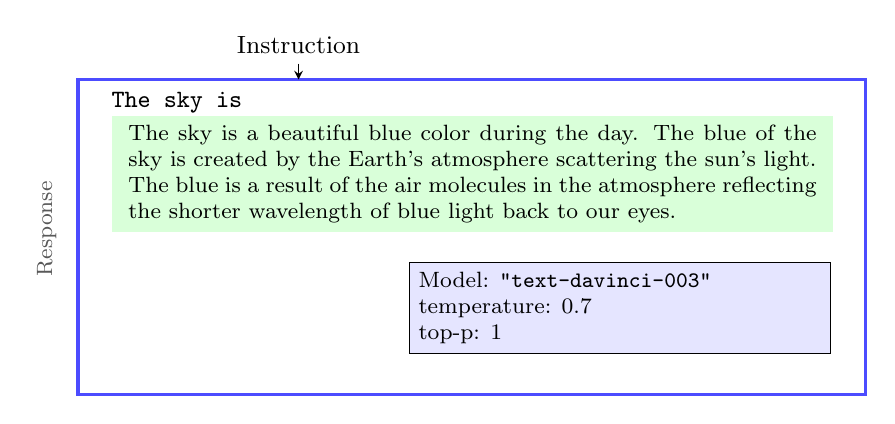
\begin{tikzpicture}[font=\small, every node/.style={align=left}]
      % Outer box (prompt/response box)
      \draw[very thick, color=blue!70] (0,0) rectangle (10,4);

      % Instruction arrow and label
      \draw[-stealth] (2.8,4.2) -- (2.8,4);
      \node[above] at (2.8,4.2) {Instruction};

      % Prompt (inside the box)
      \node[anchor=west] at (0.3,3.7) {\texttt{The sky is}};
      % Response label
      \node[rotate=90, color=gray!70!black] at (-0.4,2.1) {\footnotesize Response};

      % Green "blue" token
      \node[draw, fill=green!25, rounded corners=1pt, inner sep=1pt, text height=1.5ex] at (1.9,3.3) {\texttt{blue}};
      
      % Green box for model response
      \node[anchor=west] (resp) at (0.3,2.8) {%
        \begin{minipage}{9.2cm}
          \colorbox{green!15!white}{
            \parbox{0.95\linewidth}{%
              \footnotesize
              The sky is a beautiful blue color during the day. The blue of the sky is created by the Earth's atmosphere scattering the sun's light. The blue is a result of the air molecules in the atmosphere reflecting the shorter wavelength of blue light back to our eyes.%
            }
          }
        \end{minipage}
      };

      % Model config box
      \node[draw, fill=blue!10, anchor=west] at (4.2,1.1) {%
        \begin{minipage}{5cm}
          \footnotesize
          Model: \texttt{"text-davinci-003"}\\
          temperature: 0.7\\
          top-p: 1
        \end{minipage}
      };
    \end{tikzpicture}
  \end{center}
\end{frame}
